%/*% pdflatex -file-line-error -interaction nonstopmode %
\documentclass{article}
\usepackage{graphicx}
\graphicspath{ {./images/chaptertest/} }
\usepackage{amsmath}
\usepackage{amsfonts}
\usepackage{hyperref}
\usepackage{exercises}
\usepackage{amsthm}
\usepackage{yhmath}
\newcommand*{\oldneg}{\mathord{\sim}}

\theoremstyle{definition}
\newtheorem{definition}{Definition}

\setlength{\parindent}{.5in}
\setlength{\parskip}{12pt}

\title{Chapter Test (pg. 81)}
\begin{document}
\maketitle

\section*{1}
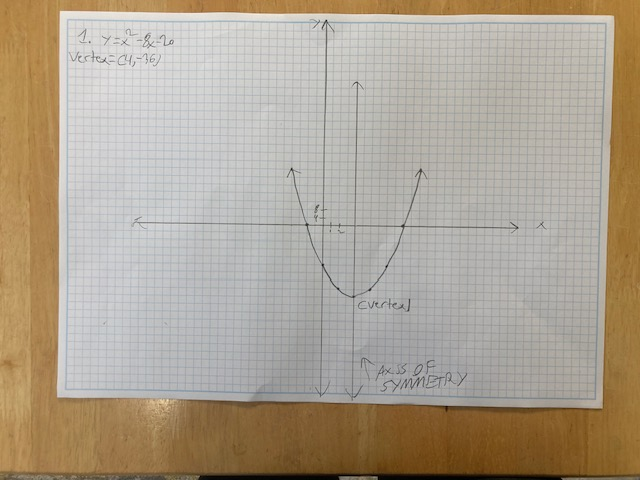
\includegraphics[width = 4in, height = 4in]{chaptertestpicture1.png}

\section*{2}
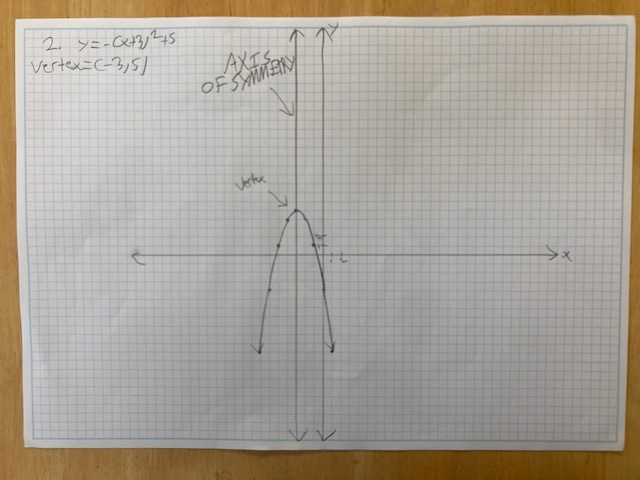
\includegraphics[width = 4in, height = 4in]{chaptertestpicture2.png}

\section*{3}
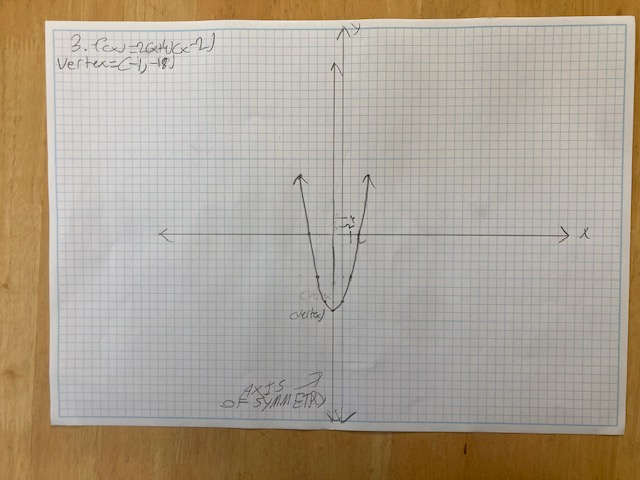
\includegraphics[width = 4in, height = 4in]{chaptertestpicture3.png}

\section*{4}
$x^2-11x+30\newline\rightarrow 
(x-6)(x-5)$

\section*{5}
$z^2+2z-15\newline\rightarrow 
(z+5)(z-3)$

\section*{6}
$n^2-64\newline\rightarrow 
(n+8)(n-8)$

\section*{7}
$2s^2+7s-15\newline\rightarrow 
(2s-3)(s+5)$

\section*{8}
$9x^2+30x+25\newline\rightarrow 
(3x)^2+30x+(5)^2\newline\rightarrow
(3x+5)^2$

\section*{9}
$6t^2+23t+20\newline\rightarrow
(3t+4)(2t+5)$

\section*{10}
$x^2-3x-40=0\newline\rightarrow 
(x-8)(x+5)=0$ (Solve by factoring)
$\newline\rightarrow x=8\vee x=-5$ (Use Zero Product Property)

\section*{11}
$r^2-13r+42=0\newline\rightarrow 
(r-7)(r-6)=0$ (Solve by factoring)
$\newline\rightarrow r=7\vee r=6$ (Use Zero Product Property)

\section*{12}
$2w^2+13w-7=0\newline\rightarrow 
(2w-1)(w+7)=0$ (Solve by factoring)
$\newline\rightarrow w=\frac{1}{2}\vee w=-7$ (Use Zero Product Property)

\section*{13}
$10y^2+11y-6=0\newline\rightarrow 
(5y-2)(2y+3)=0$ Solve by factoring)
$\newline\rightarrow y=\frac{2}{5}\vee y=-\frac{3}{2}$ (Use Zero Product Property)

\section*{14}
$2(m-7)^2=16\newline\rightarrow 
(m-7)^2=8\newline\rightarrow 
m-7=\pm\sqrt{8}$ (Solve by finding the square root)
$\newline\rightarrow m=7\pm\sqrt{8}\newline\rightarrow 
m=7\pm 2\sqrt{2}$ (Simplify the radical)

\section*{15}
$(x+2)^2-12=36\newline\rightarrow 
(x+2)^2=48\newline\rightarrow 
x+2=\pm\sqrt{48}$ (Solve by finding the square root)
$\newline\rightarrow x=-2\pm\sqrt{48}\newline\rightarrow 
x=-2\pm 4\sqrt{3}$ (Simplify the radical)

\section*{16}
$(3+4i)-(2-5i)=\newline\rightarrow 
(3-2)+(4i+5i)=1+9i$

\section*{17}
$(2-7i)(1+2i)=\newline\rightarrow 
2-7i+4i-14i^2=16-3i$

\section*{18}
$\frac{3+i}{2-3i}=\newline\rightarrow 
\frac{(3+i)(2+3i)}{(2-3i)(2+3i)}=\newline\rightarrow 
\frac{6+9i+2i+3i^2}{4+6i-6i-9i^2}=\newline\rightarrow 
\frac{6+11i+3i^2}{4-9i^2}=\newline\rightarrow 
\frac{3+11i}{13}=\newline\rightarrow 
\frac{3}{13}+\frac{11}{13}i$

\section*{19}
$x^2+4x-14=0\newline\rightarrow 
x^2+4x=14\newline\rightarrow 
x^2+4x+4=18$ (Add $(\frac{b}{2})^2$)
$\newline\rightarrow (x+2)^2=18\newline\rightarrow 
x+2=\pm\sqrt{18}\newline\rightarrow 
x=-2\pm\sqrt{18}\newline\rightarrow 
x=-2\pm 3\sqrt{2}$

\section*{20}
$x^2-10x-7=0\newline\rightarrow 
x^2-10x=7\newline\rightarrow 
x^2-10x+25=32$ (Add $(\frac{b}{2})^2$)
$\newline\rightarrow (x-5)^2=32\newline\rightarrow 
x-5\pm\sqrt{32}\newline\rightarrow 
x=5\pm\sqrt{32}\newline\rightarrow 
x=5\pm 4\sqrt{2}$

\section*{21}
$4x^2+8x+3=0\newline\rightarrow 
4(x^2+2x)=-3\newline\rightarrow 
4(x^2+2x+1)=1$ (Add $(\frac{b}{2})^2\times 4$)
$\newline\rightarrow 4(x+1)^2=1\newline\rightarrow 
(x+1)^2=\frac{1}{4}\newline\rightarrow 
x+1=\pm\sqrt{\frac{1}{4}}\newline\rightarrow 
x=-1\pm\frac{1}{2}\newline\rightarrow 
x=-\frac{1}{2}\vee x=-\frac{3}{2}$

\section*{22}
$3x^2+10x-5=0\newline\rightarrow 
x=\frac{-10\pm\sqrt{10^2-4(3)(-5)}}{2(3)}\newline\rightarrow 
x=\frac{-10\pm\sqrt{160}}{6}\newline\rightarrow 
x=\frac{-10\pm 4\sqrt{10}}{6}\newline\rightarrow 
x=\frac{-5\pm 2\sqrt{10}}{3}$

\section*{23}
$2x^2-x+6=0\newline\rightarrow 
x=\frac{1\pm\sqrt{(-1)^2-4(2)(6)}}{2(2)}\newline\rightarrow 
x=\frac{1\pm\sqrt{-47}}{4}\newline\rightarrow 
x=\frac{1\pm \sqrt{47}i}{4}\newline\rightarrow 
x=\frac{1}{4}+\frac{\sqrt{47}}{4}i\vee x=\frac{1}{4}-\frac{\sqrt{47}}{4}i$

\section*{24}
$5x^2+2x+5=0\newline\rightarrow 
x=\frac{-2\pm\sqrt{2^2-4(5)(5)}}{2(5)}\newline\rightarrow 
x=\frac{-2\pm\sqrt{-96}}{10}\newline\rightarrow 
x=\frac{-2\pm 4i\sqrt{6}}{10}\newline\rightarrow
x=\frac{-1\pm 2i\sqrt{6}}{5}\newline\rightarrow 
x=-\frac{1}{5}+\frac{2\sqrt{6}}{5}i\vee x=-\frac{1}{5}-\frac{2\sqrt{6}}{5}i$

\section*{25}
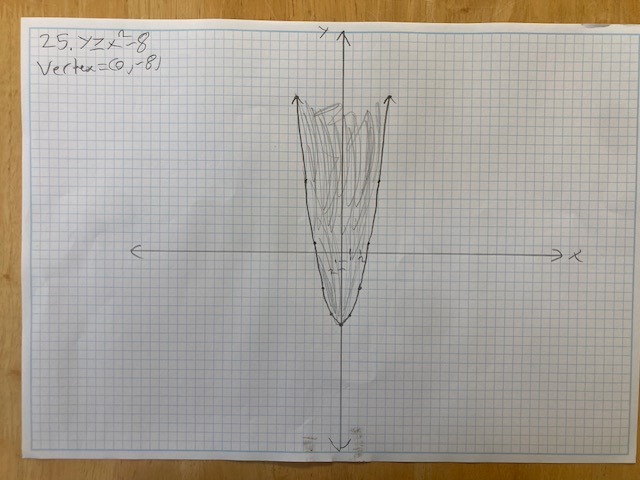
\includegraphics[width = 4in, height = 4in]{chaptertestpicture4.png}

\section*{26}
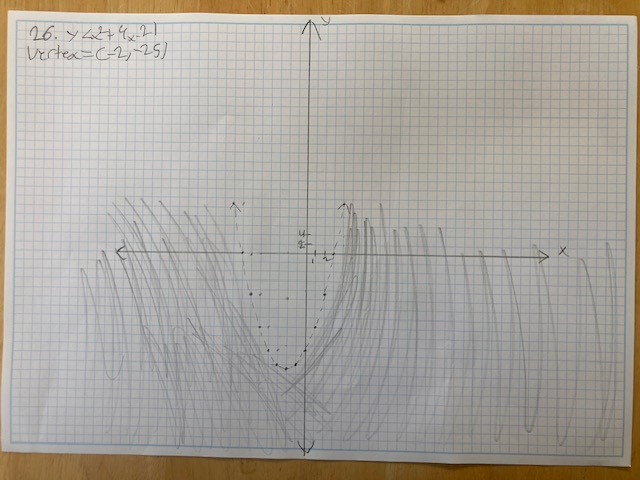
\includegraphics[width = 4in, height = 4in]{chaptertestpicture5.png}

\section*{27}
The Picture says the vertex is $(56.25)$, but I meant to say that the vertex is $(2.5,56.25)$.
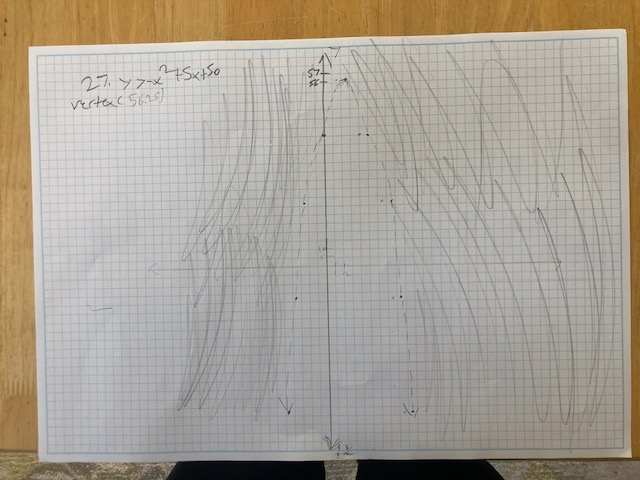
\includegraphics[width = 4in, height = 4in]{chaptertestpicture6.png}

\section*{28}
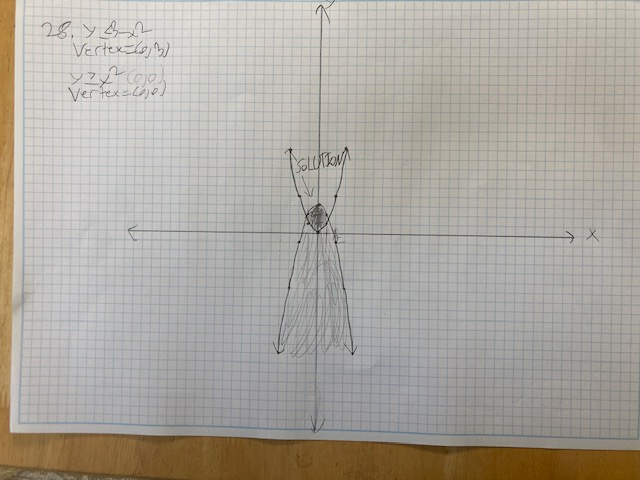
\includegraphics[width = 4in, height = 4in]{chaptertestpicture9.png}

\section*{29}
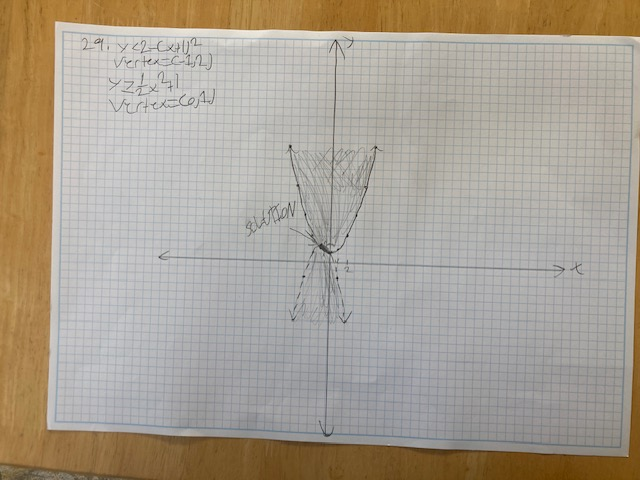
\includegraphics[width = 4in, height = 4in]{chaptertestpicture8.png}

\section*{30}
The picture says it is problem 27, but it is acutally problem 30.\newline
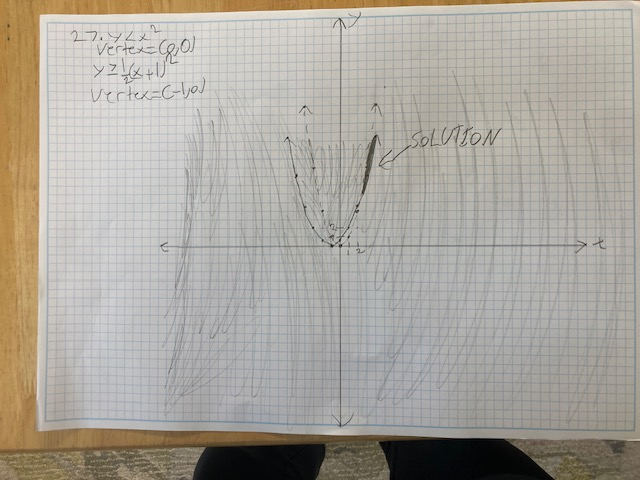
\includegraphics[width = 4in, height = 4in]{chaptertestpicture7.png}

\section*{31}
By the pythagorean theorem, we know that in a right triangle, $a^2+b^2=c^2$. When observing the given diagram, we can tell that $c=32,a=9x,b=16x$. Thus, 
$32^2=(9x)^2+(16x)^2\newline\rightarrow 
1024=81x^2+256x^2\newline\rightarrow 
1024=337x^2\newline\rightarrow 
x^2=\frac{1024}{337}\newline\rightarrow 
x=\pm\frac{\sqrt{1024}}{\sqrt{337}}\newline\rightarrow 
x=\pm\frac{\sqrt{1024}\sqrt{337}}{\sqrt{337}\sqrt{337}}$ (Simplify the radical)
$\newline\rightarrow x=\pm\frac{\sqrt{345088}}{337}\newline\rightarrow 
x=\pm\frac{32\sqrt{337}}{337}\newline$ Because it does not make sense to have $x$ be negative (if this were the case, then we would have negative 
measurements), $x$ must be positive, meaning $x=\frac{32\sqrt{337}}{337}$
\end{document}
